% Copyright 2018-2021 Melvin Eloy Irizarry-Gelpí
\setcounter{chapter}{6}
\chapter{Thin Lenses}
%
In this experiment you will learn about the properties of images produced by thin lenses.
%
\section{Preliminary}
%
Mirrors can be used to redirect the path of light rays. When a ray encounters a mirror, it bounces off. Lenses can also be used to change the direction of light rays. However, a lens uses a different mechanism called \textbf{refraction}.

Refraction is what happens when a ray of light crosses the boundary between two different materials. For example, a light ray traveling through air and encountering a piece of glass. As the ray crosses from air to glass, its direction of travel changes.

Just like for mirrors, the size and shape of a lense affects how it refracts rays of light. You can have \textbf{concave}, \textbf{convex}, or \textbf{planar} (flat) lenses. In the previous experiment, you produced a real image on a screen with a concave mirror. Here you are going to use \textbf{convex lenses} to also produce real images. Strictly speaking, the lenses that you are going to use are \textbf{double convex lenses}, meaning that both the side where light enters the lens, and the side where light exits the lens, are convex.

As for mirrors, you have the distance between the object and the lens ($d_{\text{O}}$), the distance between the image and the lens ($d_{\text{I}}$), and the focal length of the lens ($f$). These three quantities are related via
\begin{equation}
    \frac{1}{d_{\text{O}}} + \frac{1}{d_{\text{I}}} = \frac{1}{f}
\end{equation}
This is the same relation that you found to hold for the concave mirror.

The image produce by the double convex lens might have a different size and orientation as the object, so it is useful again to work with the \textbf{magnification} quantity:
\begin{equation}
    m = \frac{h_{\text{I}}}{h_{\text{O}}} = \frac{d_{\text{I}}}{d_{\text{O}}}
\end{equation}
Here, as before, $h_{\text{I}}$ is the height of the image, and $h_{\text{O}}$ is the height of the object.
%
\section{Experiment}
%
The experiment with the convex lens is very similar to the experiment done with the concave mirror. The only difference is that, since the image from the convex lens is behind the lens, you can use a full screen to project the image instead of the half-screen used before with the mirror. You have two convex lenses available, so you can measure the focal length of each.
%
\section{Analysis}
%
Although the experiment is slightly different, the analysis of the data is exactly the same as done for the concave mirror data. With the position of the object ($x_{\text{O}}$), the position of the lens ($x_{\text{L}}$), and the position of the image ($x_{\text{I}}$), you can calculate the two relevant distances:
\begin{align}
    d_{\text{O}} = \left\vert x_{\text{O}} - x_{\text{L}} \right\vert && d_{\text{I}} = \left\vert x_{\text{I}} - x_{\text{L}} \right\vert
\end{align}
The chart with $1/d_{\text{I}}$ in the vertical axis, and $1/d_{\text{O}}$ in the horizontal axis should have a linear shape. The \textbf{slope} should be:
\begin{equation}
    \text{slope} = -1
\end{equation}
The \textbf{intercept} should correspond to the \textbf{inverse of the focal length} of the lens:
\begin{equation}
    \text{intercept} = \frac{1}{f}
\end{equation}
Taking the inverse gives the focal length:
\begin{equation}
    f = \frac{1}{\text{intercept}}
\end{equation}
You can do this for both lenses. You can also calculate the magnification in two different ways and show that both ways are essentially equivalent.
%
\section{My Data}
%
My data consist of more measurements at different positions than the ones suggested in class. As you can see from Figure \ref{figure.08.10cm} and Figure \ref{figure.08.20cm}, the relation between the inverse distances to the lens is observed. The results are in Table \ref{table.08.results}, and are very close to the expected value.

The magnification can be calculated in two ways. Instead of using height, I used \textbf{width}. In the end it does not matter, as long as you are consistent (in the sense that you cannot divide a height by a width). As can be seen from Table \ref{table.08.magnification.10cm} and \ref{table.08.magnification.20cm}, both ways of calculating magnification give similar results. However, it was hard to accurately measure the size of the smaller images. This is reflected in repeated values for the width. In this sense, the distance measurements provide a more refined way of estimating the magnification.
%
\section{Your Data}
%
You should have positions and heights for both double convex lenses.
%
% \newpage
% \section{Your Report}
% %
% Your report should include the following:
% \begin{itemize}
%     \item Tables like Table \ref{table.08.position.10cm} and \ref{table.08.position.20cm} with the raw position data for both lenses.
%     \item Tables like Table \ref{table.08.magnification.10cm} and \ref{table.08.magnification.20cm} with the calculated magnification using the size and also distance.
%     \item Figures like Figure \ref{figure.08.10cm} and \ref{figure.08.20cm} with the inverse distance data. Include the best-fit line and display the equation.
%     \item A table like Table \ref{table.08.results} with your results for the slope and the focal length for each lens. Include the percent difference.
%     \item Answer the following question: Which approach to calculating the magnification is more accurate and why?
% \end{itemize}
%
\newpage
\section{Tables}
%
\begin{table}[ht]
    \centering
    \begin{tabular}{|r|r|r|}
        \hline
        $x_{\text{O}}$ (cm) & $x_{\text{L}}$ (cm) & $x_{\text{I}}$ (cm) \\
        \hline
        10 & 25 & 56.9 \\
        10 & 30 & 51.4 \\
        10 & 35 & 52.6 \\
        10 & 40 & 55.3 \\
        10 & 45 & 59.5 \\
        10 & 50 & 63.6 \\
        10 & 55 & 68 \\
        10 & 60 & 72.8 \\
        10 & 65 & 77.7 \\
        10 & 70 & 82.5 \\
        \hline
        \end{tabular}
    \caption{Raw Position Data for 10 cm Double Convex Lens}
    \label{table.08.position.10cm}
\end{table}
%
\begin{table}[ht]
    \centering
    \begin{tabular}{|r|r|}
        \hline
        $w_{\text{I}}$ (cm) & $w_{\text{O}}$ (cm) \\
        \hline
        3.8 & 2 \\
        2 & 2 \\
        1.4 & 2 \\
        1 & 2 \\
        0.8 & 2 \\
        0.6 & 2 \\
        0.4 & 2 \\
        0.4 & 2 \\
        0.4 & 2 \\
        0.3 & 2 \\
        \hline
    \end{tabular}
    \caption{Raw Width Data for 10 cm Double Convex Lens}
    \label{table.08.width.10cm}
\end{table}
%
\begin{table}[ht]
    \centering
    \begin{tabular}{|r|r|}
        \hline
        $w_{\text{I}} / w_{\text{O}}$ & $d_{\text{I}} / d_{\text{O}}$ \\
        \hline
        1.9 & 2.127 \\
        1 & 1.070 \\
        0.7 & 0.704 \\
        0.5 & 0.510 \\
        0.4 & 0.414 \\
        0.3 & 0.340 \\
        0.2 & 0.289 \\
        0.2 & 0.256 \\
        0.2 & 0.231 \\
        0.15 & 0.208 \\
        \hline
    \end{tabular}
    \caption{Magnification for 10 cm Double Convex Lens}
    \label{table.08.magnification.10cm}
\end{table}
%
\begin{table}[ht!]
    \centering
    \begin{tabular}{|r|r|r|}
        \hline
        $x_{\text{O}}$ (cm) & $x_{\text{L}}$ (cm) & $x_{\text{I}}$ (cm) \\
        \hline
        5 & 30.7 & 120 \\
        5 & 94.1 & 120 \\
        10 & 36.4 & 120 \\
        10 & 93.4 & 120 \\
        15 & 42 & 120 \\
        15 & 93.1 & 120 \\
        20 & 47.5 & 120 \\
        20 & 92.6 & 120 \\
        25 & 53.6 & 120 \\
        25 & 91.1 & 120 \\
        30 & 59.8 & 120 \\
        30 & 89.1 & 120 \\
        35 & 67.6 & 120 \\
        35 & 87.6 & 120 \\
        \hline
        \end{tabular}
    \caption{Raw Position Data for 20 cm Double Convex Lens}
    \label{table.08.position.20cm}
\end{table}
%
\begin{table}[ht]
    \centering
    \begin{tabular}{|r|r|}
        \hline
        $w_{\text{I}}$ (cm) & $w_{\text{O}}$ (cm) \\
        \hline
        6.3 & 2 \\
        0.6 & 2 \\
        5.8 & 2 \\
        0.6 & 2 \\
        5.4 & 2 \\
        0.7 & 2 \\
        4.8 & 2 \\
        0.8 & 2 \\
        4.1 & 2 \\
        0.7 & 2 \\
        3.6 & 2 \\
        0.9 & 2 \\
        2.9 & 2 \\
        1.4 & 2 \\
        \hline
    \end{tabular}
    \caption{Raw Width Data for 20 cm Double Convex Lens}
    \label{table.08.width.20cm}
\end{table}
%
\begin{table}[ht]
    \centering
    \begin{tabular}{|r|r|}
        \hline
        $w_{\text{I}} / w_{\text{O}}$ & $d_{\text{I}} / d_{\text{O}}$ \\
        \hline
        3.15 & 3.475 \\
        0.3 & 0.291 \\
        2.9 & 3.167 \\
        0.3 & 0.319 \\
        2.7 & 2.889 \\
        0.35 & 0.344 \\
        2.4 & 2.636 \\
        0.4 & 0.377 \\
        2.05 & 2.322 \\
        0.35 & 0.437 \\
        1.8 & 2.020 \\
        0.45 & 0.523 \\
        1.45 & 1.607 \\
        0.7 & 0.616 \\
        \hline
    \end{tabular}
    \caption{Magnification for 20 cm Double Convex Lens}
    \label{table.08.magnification.20cm}
\end{table}
%
\begin{table}[ht]
    \centering
    \begin{tabular}{|l|r|r|r|}
        \hline
        Name & Expected Value & Observed Value & P.D. (\%) \\
        \hline
        Slope for 10 cm Double Convex Lens & \textminus 1 & \textminus 1.004 & 0.04 \\
        $f$ for 10 cm Double Convex Lens & 10 cm & 10.22 cm & 2.19 \\
        Slope for 20 cm Double Convex Lens & \textminus 1 & \textminus 0.992 & \textminus 0.84 \\
        $f$ for 20 cm Double Convex Lens & 20 cm & 20.13 cm & 0.64 \\
        \hline
    \end{tabular}
    \caption{Results}
    \label{table.08.results}
\end{table}
%
\FloatBarrier
\newpage
\section{Figures}
%
\begin{figure}[ht]
    \centering
    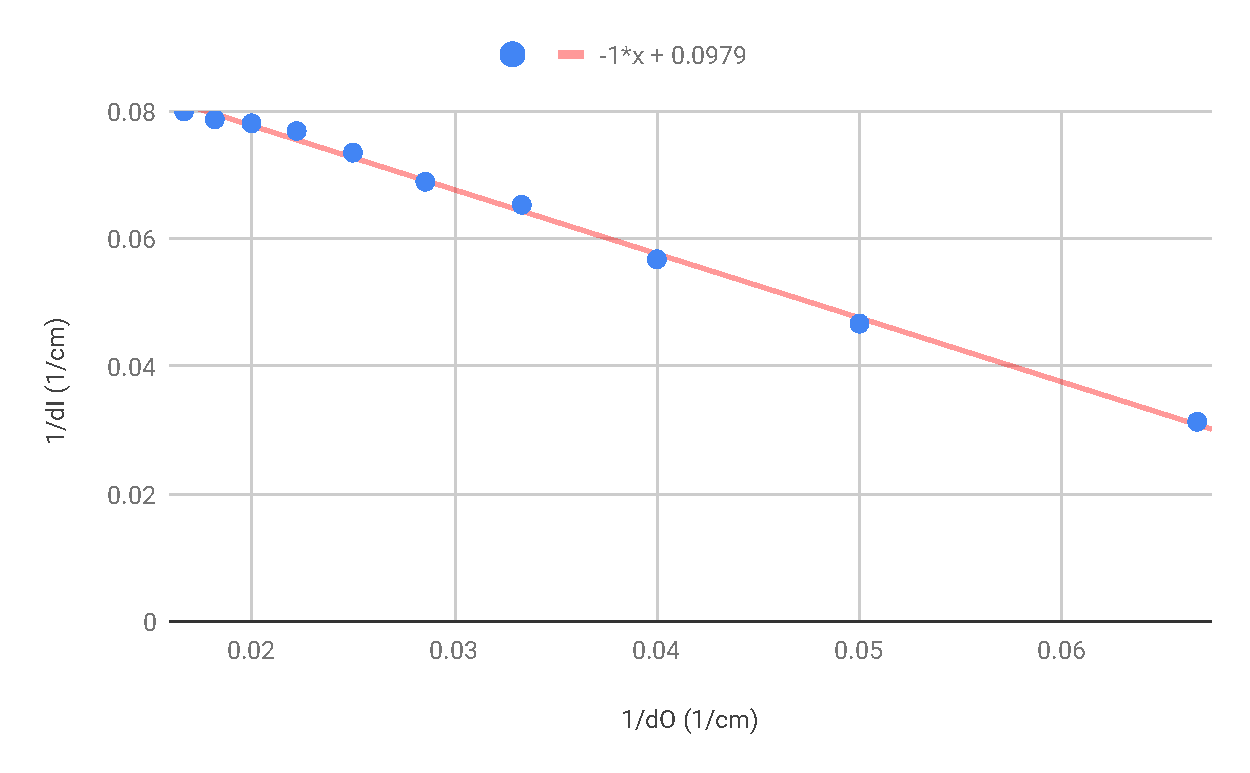
\includegraphics[scale=0.74]{image/08-lenses/10cm.pdf}
    \caption{Linear Fit for 10 cm Double Convex Lens}
    \label{figure.08.10cm}
\end{figure}
%
\begin{figure}[ht]
    \centering
    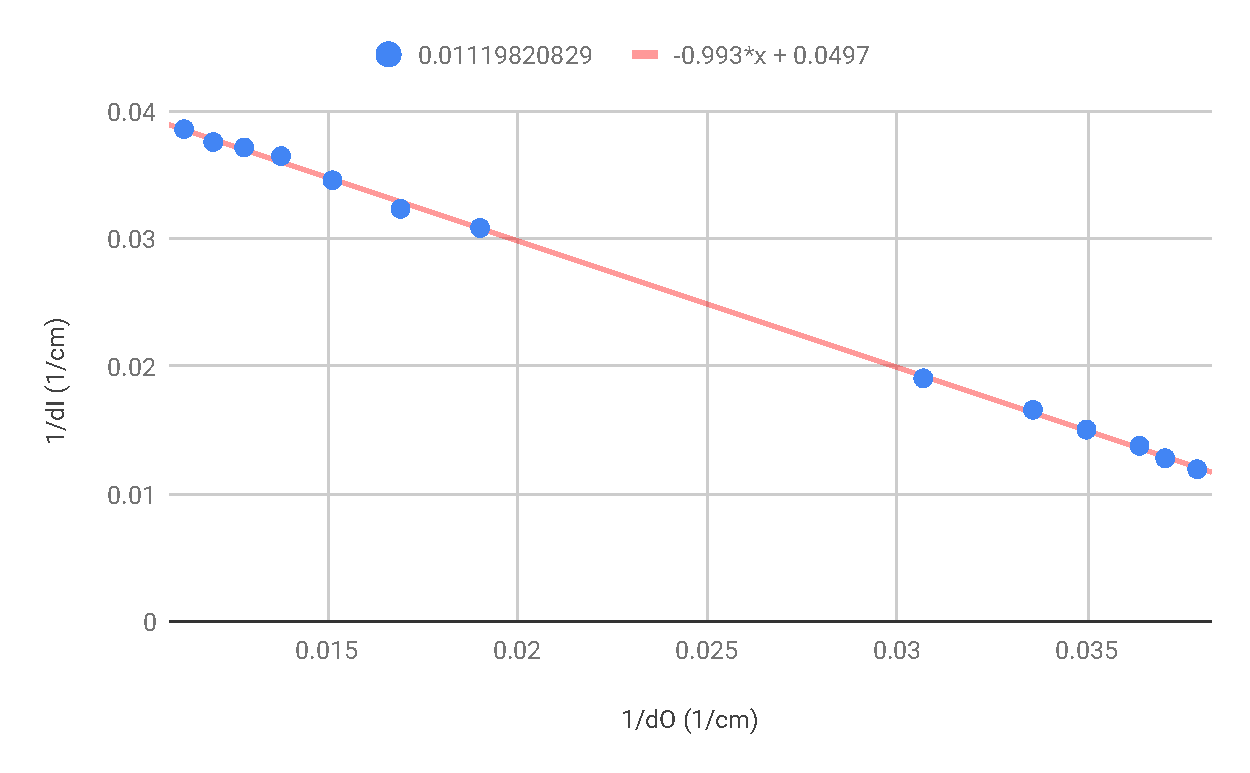
\includegraphics[scale=0.74]{image/08-lenses/20cm.pdf}
    \caption{Linear Fit for 20 cm Double Convex Lens}
    \label{figure.08.20cm}
\end{figure}
%